\documentclass[11pt, a4paper]{article}

% Essential packages
\usepackage[margin=1in]{geometry}
\usepackage[utf8]{inputenc}
\usepackage[T1]{fontenc}
\usepackage[english]{babel}
\usepackage{amsmath}
\usepackage{amssymb}
\usepackage{graphicx}
\usepackage{booktabs}
\usepackage{microtype}
\usepackage{hyperref}
\usepackage{cite}
\usepackage{caption}
\usepackage{enumitem}
\usepackage{longtable}

% Global formatting
\captionsetup{font=small, labelfont=bf, skip=6pt}
\setlist[itemize]{leftmargin=1.5em, itemsep=0.3em, topsep=0.4em}
\setlength{\LTpre}{0.75em}
\setlength{\LTpost}{0.75em}
\renewcommand{\arraystretch}{1.1}
\hypersetup{
    colorlinks=true,
    linkcolor=black,
    citecolor=black,
    urlcolor=blue
}

% Document metadata
\title{The Impact of Short-term Intensity and Tactical Behavior on Goal-Scoring Probability: A Machine Learning Approach}

\author{
    Jakub Piotrowski \and Jakub Szulc \and Mateusz Jastrzębski \\
    \vspace{0.2cm}
    \textit{Polish-Japanese Academy of Information Technology}
}
\date{\today}

\begin{document}

\maketitle

\begin{abstract}
Football data analysis has evolved significantly—from coaches' intuition and manual match decomposition to advanced statistical methods—yet most approaches universally rely on broader contextual evaluations of player performance. Currently, predictive models typically analyze a player's behavior by incorporating historical match data and the relative strengths of competing teams. However, predicting the probability of scoring a goal based strictly on real-time, isolated in-match performance remains a largely unexplored area. To address this gap, we developed machine learning models trained on behavioral data from 31 fixtures, segmented into 15-minute intervals. The feature set included high-intensity stress moments, distance covered, shot volume and technique, behavior under pressure, passing phases, as well as formation and positioning. We used \textbf{fixture-grouped, stratified 3-fold cross-validation} and evaluated \textbf{out-of-fold (OOF)} predictions from logistic regression, Extra Trees, Random Forest, XGBoost, and LightGBM. A \textbf{stacking} ensemble combined these base models by training a \textbf{meta--logistic regressor} on the OOF probability vectors (with optional probability calibration and fold-wise F1-tuned decision rules). The strongest single OOF model by PR-AUC was \textbf{Random Forest} (ROC-AUC $\approx$~0.679, PR-AUC $\approx$~0.120; Brier $\approx$~0.058), while the stacked ensemble achieved a slightly \textbf{higher ROC-AUC} ($\approx$~0.682) and better ranked minority detection than several tree baselines at the cost of a lower PR-AUC ($\approx$~0.114) in this run. We additionally report an \textbf{AutoGluon} holdout benchmark on a single train/validation split of the all-features matrix (not directly comparable to full-dataset OOF). Despite a highly imbalanced dataset (about 94\% negative, 6\% positive at checkpoints on pitch), the models improved ranking over the base rate, but absolute PR-AUCs remain low---consistent with a rare, noisy label. Overall, a player's recent 15-minute activity and cumulative in-match state carry measurable signal, but isolated in-game tabular features alone are insufficient for high-confidence individual goal forecasting without richer context.
\end{abstract}

\section{Introduction}

Football data analysis has undergone a profound transformation over the last decade. Moving beyond traditional coaches' intuition and manual match decomposition, the field has embraced advanced statistical methods and machine learning. Modern tactical analytics heavily rely on complex data streams, including spatial tracking and detailed behavioral event logs. Within this domain, predicting key match events—most notably, goal-scoring—remains the holy grail of sports analytics, offering invaluable insights for real-time tactical adjustments and decision-making.

Currently, the majority of predictive models in football evaluate player performance through a broad, historical lens. Frameworks such as Expected Goals (xG) excel at quantifying the quality of an isolated shot, while broader match-outcome models heavily depend on cumulative metrics, such as a player's season-long statistics, historical Elo ratings, and the relative strength of the opposing team. While these approaches provide a comprehensive macro-perspective, they inherently dilute the impact of immediate, in-game dynamics. 

This reveals a significant gap in the current literature: the evaluation of goal-scoring probability based strictly on a player's real-time, isolated performance during a match. The fundamental question arises whether short-term physical and tactical intensity—such as behavior under defensive pressure, sprint frequency, and passing phases—can serve as an independent predictive signal, stripped of external historical context. Specifically, it remains largely unexplored whether a player's isolated activity in recent 15-minute intervals can accurately forecast their likelihood of scoring later in the game.

To address this gap, this paper proposes a machine learning approach focused exclusively on in-match player behavior. We formulate the problem using tabular data extracted from 31 professional fixtures during the UEFA Under-21 European Championship held in Slovakia in 2025, segmenting player activity into 15-minute checkpoints. To capture complex, non-linear relationships within the data, we implemented a \textbf{stacking} architecture on \textbf{OOF} predictions from several base learners, plus an optional \textbf{AutoGluon} holdout run for an alternative ensemble perspective. A critical aspect of our methodology is the rigorous feature engineering process, designed to strictly prevent target leakage across temporal windows: events are compared to checkpoints using \textbf{absolute} match time, and we exclude substitution-timing fields that encode future information from modeling features (e.g., \texttt{minute\_out} and \texttt{subbed}) in the main pipeline, following the project implementation.

The main contributions of this paper are summarized as follows:
\begin{itemize}
    \item \textbf{Novel Temporal Data Representation:} We introduce a checkpoint-based methodology that isolates short-term (15-minute) and cumulative in-match player performance, effectively separating real-time form from historical bias, with fold-safe feature construction.
    \item \textbf{Robust Predictive Modeling:} We developed a stacking ensemble for highly imbalanced sports data, with grouped cross-validation to prevent match-level leakage, and we report OOF metrics alongside an optional AutoGluon holdout.
    \item \textbf{Behavioral Insights:} We provide a feature analysis identifying which on-field behaviors most strongly align with the learned models (e.g., territorial pass shares, HSR, pressure-quality proxies), with importance estimates derived from the same fold-safe feature matrix used in evaluation.
\end{itemize}

\section{Related Work}

The application of statistical modeling and machine learning in football has expanded rapidly, primarily focusing on event valuation and macro-level match forecasting. 

\textbf{Event Valuation Models.} The cornerstone of modern football analytics is the Expected Goals (xG) framework, which quantifies the probability of a shot resulting in a goal based on historical and spatial context. Extending this logic beyond shooting, models like Expected Threat (xT) \cite{singh2019xt} evaluate the probability of scoring based on how ball progression (e.g., passes and carries) shifts the game state into more dangerous zones. While these models are highly effective at evaluating specific actions retrospectively, they are fundamentally reactive. They evaluate the \textit{outcome} of an event rather than forecasting the \textit{future onset} of a scoring opportunity based on the physical and tactical intensity leading up to it.

\textbf{Match Outcome Prediction.} Another significant branch of literature focuses on predicting broader match outcomes (win, draw, loss) using machine learning algorithms such as Random Forest \cite{breiman2001random} and XGBoost \cite{chen2016xgboost}. These studies typically rely on aggregated pre-match features, including season-long team statistics, historical Elo ratings, and betting odds. While these macroscopic approaches achieve reasonable accuracy, they inherently obscure the micro-dynamics of the game. Recent studies have begun incorporating spatial tracking and physical exhaustion metrics, yet there remains a notable scarcity of research dedicated to dynamically evaluating goal-scoring probabilities for individual players using strictly isolated, short-term temporal windows (e.g., 15-minute checkpoints). Our work directly addresses this gap by shifting the predictive focus from global match states to real-time, player-specific tactical behaviors.

\section{Methodology}

The methodology section outlines the data processing pipeline, the temporal feature engineering framework, the model architecture, and the rigorous validation strategy designed to predict the rare event of a player scoring a goal.

\subsection{Data Collection and Preprocessing}

The primary dataset defines a rare-event, player-checkpoint prediction problem based on the UEFA Under-21 European Championship 2025. The core modeling table consists of 3,486 checkpoint observations across 31 fixtures, encompassing 307 unique players and 869 player appearances. The target variable, indicating whether a player scores after a 15-minute checkpoint, exhibits class imbalance: in the modeling run summarized here, 203 positive checkpoints against 3,283 negatives on-pitch, yielding a base positive rate of 5.82\%.

\begin{longtable}{lrrlp{0.34\linewidth}}
\caption{Dataset overview including the main modeling table and supplemental event logs (row and appearance counts as in the source CSVs).}
\label{tab:dataset_overview} \\
\toprule
Dataset & Rows & Approx.\ columns$^*$ & Unique player appearances in file & Role \\
\midrule
Checkpoints & 3,486 & 33 & 869 & Main modeling table \\
Passes & 29,795 & 7 & 959 & Passing event context \\
Runs & 35,133 & 10 & 968 & Physical event context \\
Shots & 780 & 12 & 453 & Attacking event context \\
Pressure & 12,185 & 10 & 923 & Pressed-action context \\
\bottomrule
\end{longtable}
{\footnotesize $^*$Column counts are from raw CSVs; the engineered modeling table uses hundreds of derived features after folding and encoding.}

\begin{longtable}{lrrr}
\caption{Target distribution across different metrics (checkpoint-level, from exploratory summaries aligned with the modeling table).}
\label{tab:target_distribution} \\
\toprule
Segment & Observations & Positives & Positive rate \\
\midrule
All checkpoints (modeling table) & 3,486 & 203 & 5.82\% \\
Home players & 1,744 & 91 & 5.22\% \\
Away players & 1,742 & 112 & 6.43\% \\
\bottomrule
\end{longtable}

To provide tactical context, the checkpoints were enriched with event-level data, including 29,795 passes, 35,133 runs, 780 shots, and 12,185 pressured actions. Data cleaning focused on handling meaningful missingness. Crucially, to prevent \textbf{future} data leakage, fields such as \texttt{minute\_out} and \texttt{subbed} are excluded from the main modeling feature set in the project pipeline, because they can encode information about substitutions not guaranteed to be known at the checkpoint. The raw checkpoint column \texttt{jersey\_number} is also excluded from models to avoid spurious identity memorization; role and formation enter via engineered categoricals and frequency/target encodings when applicable.

\subsection{Feature Engineering and Temporal Representation}
The analysis treats each player-checkpoint row as a causal \emph{pre-checkpoint} information set. To capture the dynamic nature of a football match, event-derived features were constructed using a fold-safe \texttt{TemporalFeatureBuilder}. Features were organized into:
\begin{itemize}
    \item \textbf{Recent Features:} Aggregates for short windows (e.g., \texttt{last5}, \texttt{last15}) prior to the checkpoint.
    \item \textbf{Cumulative Features:} Aggregates from appearance start up to the checkpoint, plus derived rates and ratios.
\end{itemize}

Event rows were joined by \texttt{player\_appearance\_id} and filtered to events at absolute minutes not after the checkpoint; absolute time combines period and minute to avoid conflating first- and second-half minutes.

Categorical encodings, rare-level pooling, and target-rate encodings were fit \textbf{inside each training fold} before transforming validation data. The all-features ablation in the reported run used 241 raw modeling columns after a deterministic redundancy screen (duplicated or near-duplicate role/sprint/pressure/shot counts removed in favor of stable representatives).

\subsection{Model Architecture}
Given the high-dimensional, sparse, and non-linear structure of the engineered table, we prioritized tree-based models together with a linear baseline. The \textbf{base learners} in the main benchmark were: balanced logistic regression, Extra Trees, Random Forest, XGBoost, and LightGBM (all trained on the same all-features set under grouped CV; hyperparameter search for XGBoost can be enabled but was set to zero in the fast run used to refresh these numbers). 

\textbf{Stacking (OOF).} For each base model we computed \textbf{out-of-fold} predicted probabilities on all checkpoints, using the same stratified, fixture-grouped folds. A \textbf{Level-1} \texttt{LogisticRegression} with \texttt{class\_weight} balancing was fit on the matrix of OOF base probabilities, with an optional \texttt{CalibratedClassifierCV} path when it succeeds numerically, and F1-optimized decision thresholds on training folds for the reported discrete metrics.

\textbf{AutoGluon.} We additionally fit \texttt{TabularPredictor} on a \textbf{holdout} split of the all-features design matrix (first fold train vs.\ validation) with a time limit, producing an \texttt{autogluon\_holdout} row in the metrics table. This is a complementary benchmark, not a component of the OOF-stacking vector above.

\subsection{Validation Strategy and Evaluation Metrics}
A standard random row split would leak shared match state across train and test. We used \textbf{stratified grouped} cross-validation with groups defined by \texttt{fixture\_id} (3 folds in the reported run). For rare-event classification, we report ROC--AUC, PR--AUC, Brier score, and in addition precision/recall and lift-style summaries exported by the experiment runner.

\section{Experiments and Results}

\subsection{Baseline Distributions and Contextual Signals}
The overall checkpoint positive rate was 5.82\% for on-pitch rows. Exploratory rates by role (illustrative): attackers about 12.5\%, midfielders about 6.7\%, defenders about 3.0\%, goalkeepers 0.0\% in this sample—consistent with position acting as a strong first filter. By checkpoint order, the exploratory positive rate is highest in the first 15 minutes and tends to be lower in later regular-time windows, motivating explicit time/phase controls in the model.

\subsection{Model Performance (OOF, all-features set)}
Models were compared on the \texttt{all\_features} OOF probability vectors, except the AutoGluon line which is evaluated on its holdout subset (different $n$; interpret cautiously). Representative metrics are summarized in Table~\ref{tab:model_results}.

\begin{table}[h]
\centering
\caption{OOF performance on the full checkpoint table ($n=3486$), all-features, fixture-grouped CV. AutoGluon: holdout validation fold only ($n=1096$).}
\label{tab:model_results}
\begin{tabular}{lccc}
\toprule
\textbf{Model} & \textbf{ROC-AUC} & \textbf{PR-AUC} & \textbf{Brier} \\
\midrule
Stacking (OOF meta)     & 0.682 & 0.114 & 0.054 \\
Random Forest           & 0.679 & \textbf{0.120} & 0.058 \\
Extra Trees             & 0.674 & 0.113 & 0.061 \\
XGBoost                 & 0.650 & 0.107 & 0.060 \\
LightGBM                & 0.656 & 0.114 & 0.059 \\
Logistic regression     & 0.580 & 0.078 & 0.186 \\
\midrule
AutoGluon (holdout)$^\dagger$ & 0.661 & 0.080 & 0.047 \\
\bottomrule
\end{tabular}

{\footnotesize $^\dagger$Evaluated on a different sample and fixed 0.5 threshold in the export; not directly comparable to full-data OOF rows.}
\end{table}

\paragraph{Reading the table.} In this run, \textbf{Random Forest} attains the best PR-AUC among OOF baselines, while the \textbf{stacked} model achieves the highest ROC-AUC and the lowest Brier among the OOF methods compared here. The linear baseline lags the tree methods on AUC/PR, as expected, but it can still contribute positively in the meta-learner. LightGBM is competitive in PR with Extra Trees, slightly below Random Forest. AutoGluon's holdout row must not be compared naively to OOF: it uses fewer observations and a different split.

\paragraph{Meta-learner behavior (post-hoc diagnostic).} A separate linear regression on the standardized OOF columns (used only for \emph{interpretability} of stacking, not to retrain the official meta-model) places the largest positive standardized weight on \texttt{random\_forest\_all\_features}, with smaller positive weights for \texttt{extra\_trees\_all\_features} and \texttt{lightgbm\_all\_features}, and negative adjustments on \texttt{xgboost\_all\_features} and \texttt{logistic\_all\_features}---showing the meta-layer correcting systematic calibration/ranking differences between baselines.

\begin{figure}[htbp]
\centering
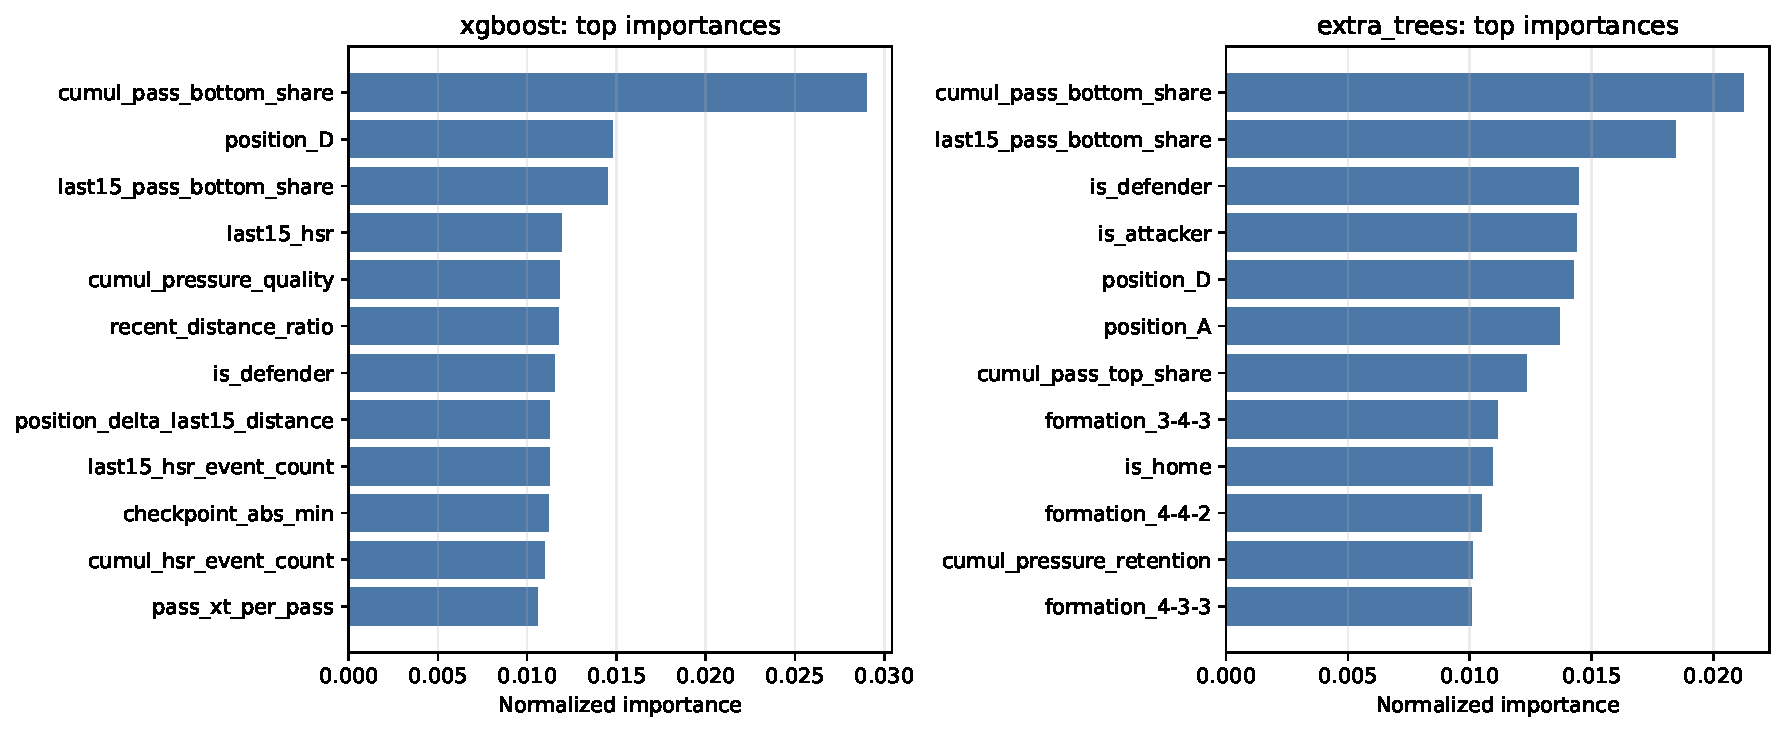
\includegraphics[width=\linewidth]{figures/model_feature_importance.pdf}
\caption{Normalized importances for selected tree-based models in the EDA/metrics export (see \texttt{reports/figures/model\_feature\_importance.csv} for the exact table used to build the figure). The production pipeline excludes substitution-timing leakage columns; any diagnostic artifact listing excluded raw fields should not override that modeling policy.}
\label{fig:feature_importance}
\end{figure}

\subsection{Feature Importance and Behavioral Insights}
We summarize normalized importances (from the same CSV that feeds Figure~\ref{fig:feature_importance}) for XGBoost and Extra Trees, rounded for presentation:

\begin{longtable}{llr}
\caption{Top normalized feature importances (selected tree-based models, from export CSV).}
\label{tab:feature_importance_summary} \\
\toprule
Model & Feature & Norm.\ importance \\
\midrule
XGBoost & \texttt{cumul\_pass\_bottom\_share} & 0.029 \\
XGBoost & \texttt{position\_D} & 0.015 \\
XGBoost & \texttt{last15\_pass\_bottom\_share} & 0.015 \\
XGBoost & \texttt{last15\_hsr} & 0.012 \\
XGBoost & \texttt{cumul\_pressure\_quality} & 0.012 \\
XGBoost & \texttt{recent\_distance\_ratio} & 0.012 \\
Extra Trees & \texttt{cumul\_pass\_bottom\_share} & 0.021 \\
Extra Trees & \texttt{last15\_pass\_bottom\_share} & 0.018 \\
Extra Trees & \texttt{is\_defender} & 0.014 \\
Extra Trees & \texttt{is\_attacker} & 0.014 \\
Extra Trees & \texttt{position\_D} & 0.014 \\
Extra Trees & \texttt{position\_A} & 0.014 \\
\bottomrule
\end{longtable}

The models emphasize territorial pass shares (defensive third involvement vs.\ high-third involvement), high-speed running in the last 15 minutes, and pressure/quality-style aggregates---alongside role indicators---consistent with the paper's earlier qualitative themes.

\begin{figure}[htbp]
\centering
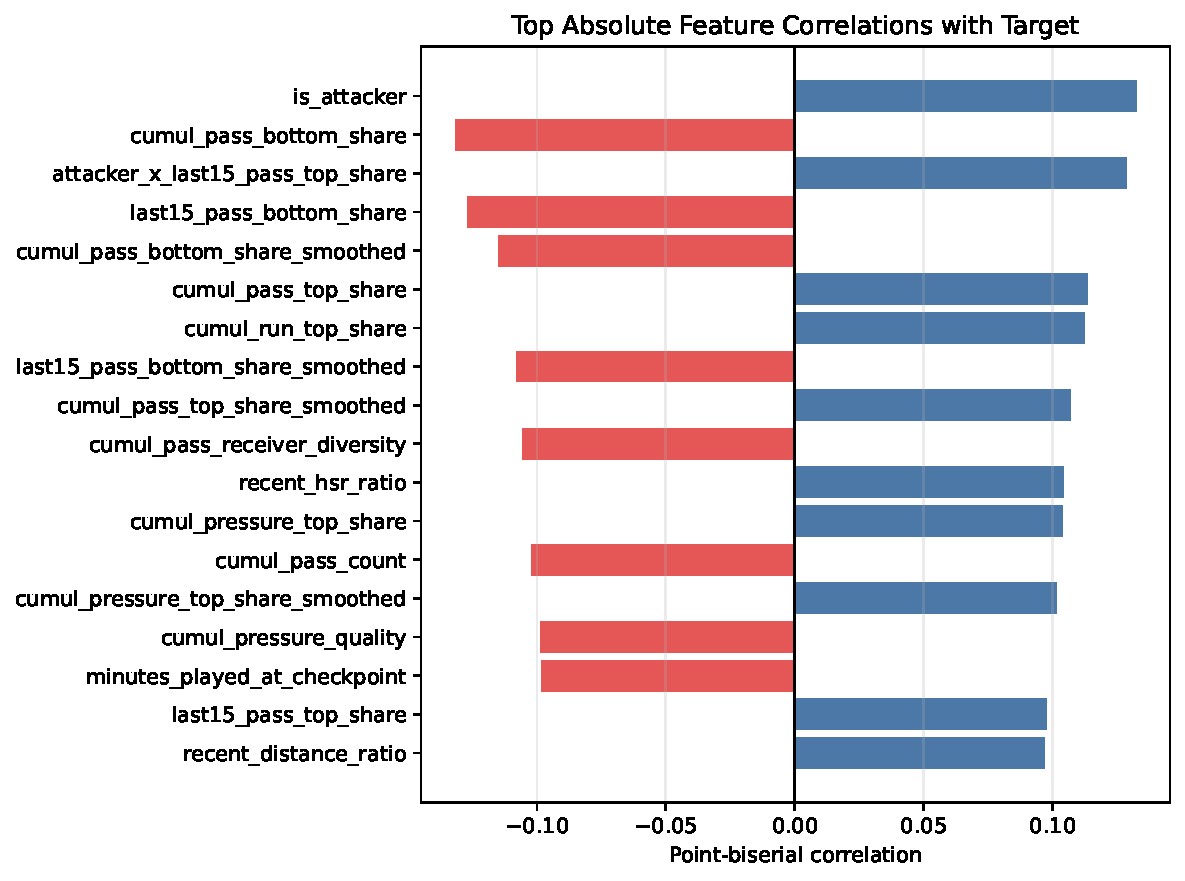
\includegraphics[width=\linewidth]{figures/feature_correlations.pdf}
\caption{Top absolute feature correlations with \texttt{scored\_after}. These are descriptive associations on the full feature matrix, not causal effects.}
\label{fig:feature_correlations}
\end{figure}

\section{Discussion}

The empirical results are modest in absolute terms (PR-AUC $\ll 0.2$), which is common for rare, highly stochastic outcomes in sport. The stacked ensemble and Random Forests improve ranking relative to a linear baseline, but no model delivers reliable individual-level event prediction from tabular in-match state alone. The most actionable interpretation is in \textbf{relative} threat ranking (lift at top deciles) and in understanding which signal families enter the model.

The strongest signals remain partly structural (role, territorial involvement), with shorter-horizon physical and pressure/quality features providing refinements. Future work, as in the conclusion below, should hybridize with macro information rather than over-interpreting marginal gains from a single run.

\section{Conclusion and Future Work}

This study examined goal-scoring prediction from strictly in-match, checkpoint-aligned behavioral and physical data. The reported experiment used grouped 3-fold OOF training with a stacking meta-learner and optional AutoGluon, yielding peak OOF PR-AUC around \textbf{0.120} and ROC-AUC up to about \textbf{0.68} in this configuration.

The most promising next step is \textbf{hybrid modeling}: combine these micro-signals with historical player and team form, match importance, and opponent strength, while preserving the same rigorous grouped validation.

\section*{Acknowledgements}

The authors would like to express their sincere gratitude to the \textbf{University of Warsaw}, the organizer of this research initiative, for providing the structural support and the framework necessary for this study. Furthermore, we acknowledge the providers of the UEFA Under-21 European Championship 2025 dataset, which served as the empirical basis for this work.

% Bibliography
\bibliographystyle{plain}
\bibliography{references} % Provide references.bib in the same directory (or set path) when compiling

\end{document}
